\chap{Zusammenfassung der VPL-Blöcke}\label{a.blocks}

\sect{Ereignisblöcke}

\blksm{event-buttons} \textbf{Buttons}. Klickt man auf einen oder mehrere der Knöpfe im abgebildeten Block, werden diese rot. Ein Ereignis tritt ein, wenn die roten Knöpfe betätigt werden. 

\bigskip\bigskip


\blksm{event-prox} \textbf{Horizontale Distanzsensoren} (fünf vorne und zwei hinten). Klickt man auf eines oder mehrere der kleinen Quadrate im abgebildeten Block, ändern diese ihre Farbe. Zu Beginn sind alle Quadrate grau, was bedeutet, dass die Sensoren ignoriert werden. 

Wenn das Quadrat weiss mit rotem Rand ist \blksm{center-prox}, tritt ein Ereignis ein, wenn dort viel Licht reflektiert wird. 

Wenn das Quadrat schwarz ist \blksm{center-no-prox}, tritt ein Ereignis ein, wenn dort sehr wenig Licht reflektiert wird. 

\bigskip

\trickbox{Gewöhnliche Objekte müssen sehr Nahe sein, um von Thymio erkannt zu werden. Sie können die Reichweite stark ausweiten, wenn Sie \emph{Reflexstreifen} an dem Objekt befestigen, welche man bei Fahrrädern einsetzt.\footnote{Danke an Francesco Mondada für diesen Tipp!}\\
Vergleichen sie folgendes Bild mit der \cref{fig.cat-mouse}:
\begin{center}
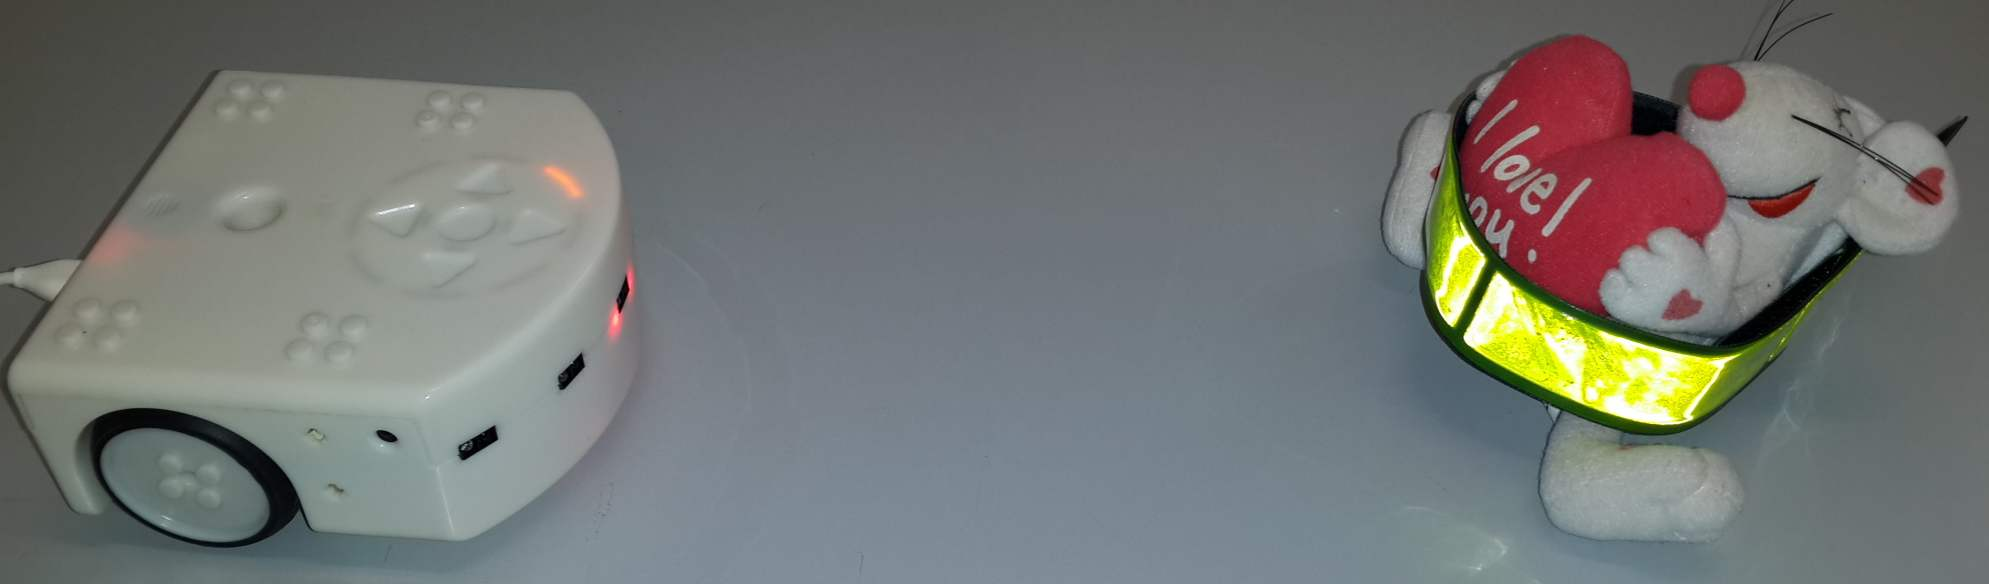
\includegraphics[width=0.8\textwidth]{reflect}
\end{center}
}

\bigskip

\blksm{event-prox-ground} \textbf{Bodendistanz-Sensoren} (zwei auf der Unterseite von 
Thymio). Gleiche Verwendung wie die horizontalen Distanzsensoren.

\bigskip\bigskip

\blksm{event-prox-advanced}, \blksm{event-prox-ground-advanced}
\textbf{Sensoren im Fortgeschrittenen Modus}. Gleiche Verwendung wie bei den vorigen Blöcken. Der obere Schieberegler legt für den rot umrahmten Sensor fest, ab wann das Ereignis eintritt (Grenzwert). Der untere Schieberegler legt für den schwarzen Sensor fest, bis zu welchem Grenzwert das Ereignis des Nicht-Erkennens eintritt.  

\bigskip\bigskip

Es gibt für das Sensorquadrat noch eine weitere Farbe im Fortgeschrittenen-Modus: dunkelgrau \blksm{slow-mid}; hier sind beide Schieberegler aktiv und man legt den Bereich des das Ereignis auslösenden Bereichs mittels Obergrenze und Untergrenze des Grenzwerts fest. 

\bigskip\bigskip\bigskip

\blksm{event-tap} \textbf{Klopfen}. Ein Ereignis tritt ein, wenn man auf den Thymio klopft. 

\bigskip\bigskip\bigskip

\blksm{event-tap-advanced} \textbf{Klopfen, Fortgeschrittener-Modus}. Gleicher Einsatz wie im Standard-Modus. Um die Beschleunigungssensoren zu aktivieren, muss der mittlere oder rechte Kreis ausgewählt werden. 

\bigskip\bigskip

\blksm{event-roll}, \blksm{event-pitch} \textbf{Beschleunigungssensor, Fortgeschrittener Modus}. Ziehen Sie das weisse Winkel-Segment im Halbkreis nach links oder rechts. Ein Ereignis tritt ein, wenn der entsprechende Winkel links / rechts bzw. vorwärts / rückwärts mit der Lage des Roboters übereinstimmt. 

\bigskip\bigskip\bigskip\bigskip

\blksm{event-timer} \textbf{Timer, Fortgeschrittener Modus}. Ein Ereignis tritt ein, wenn der Timer bei Null angelangt ist. Der Timer muss durch eine vorgängige Timer-\emph{Aktion} gesetzt werden.

\bigskip\bigskip\bigskip

\blksm{event-state} \textbf{Zustands-Ereignis, Fortgeschrittener Modus}. Das Ereignis tritt nur ein, wenn die Komponenten des aktuellen Zustands mit den entsprechenden weissen und orangen Vierteln dieses Blocks übereinstimmen. Die Komponenten, die den grauen Vierteln entsprechen, müssen nicht übereinstimmen. 

\bigskip

\sect{Aktions-Blöcke}

\blksm{action-motors} \textbf{Motoren}. Bewegen Sie den linken und rechten Schieberegler nach oben oder unten um die gewünschte Bewegung zu erreichen (links = linkes Rad, rechts = rechts Rad; oben = vorwärts, je höher desto schneller - analog unten für rückwärts). 

\newpage

\blksm{action-colors-up} \textbf{Obere Lichter}. Schieben Sie die drei Schieberegler nach rechts, um den Farbanteil von rot, grün und blau anzupassen. 

\bigskip\bigskip

\blksm{action-colors-down} \textbf{Untere Lichter}. Schaltet die unteren Lichter ein; Verwendung wie beim vorherigen Block. 

\bigskip\bigskip

\blksm{action-music} \textbf{Musik}. Die sechs kleinen Kreise sind Noten. Ein schwarzer Kreis steht für eine kurze Note, ein weisser für eine lange, ein leerer (unsichtbarer) Kreis bedeutet eine Pause. Klicken Sie auf den Kreis, um die Dauer zu ändern, klicken (oder ziehen) Sie auf die Linien, um die Tonhöhe zu ändern. 

\bigskip\bigskip

\blksm{action-timer} \textbf{Timer, Fortgeschrittener Modus} Der Timer kann für eine Zeit von bis zu 4 Sekunden eingestellt werden. Klicken Sie innerhalb des weissen Kreises (Uhr), um den Timer zu setzen. Es erscheint dann eine kurze Animation und die Dauer des Timers wird blau dargestellt. 

\bigskip\bigskip

\blksm{action-states} \textbf{Zustände, Fortgeschrittener Modus} Die vier Viertel im Block entsprechen den vier Komponenten des Zustands. Klicken Sie ein Viertel an, um die Farbe auf grau, orange bzw. weiss zu ändern. 

\sect{Hinweise zu den VPL-Blöcken}

\informationbox{Drehen an Ort oder sanfte Wende}{Wenn die Motoren bei gleicher Geschwindigkeit in die Gegenrichtung drehen, dreht der Roboter an Ort. Wird nur ein Motor eingeschaltet, fährt der Roboter und wendet sich dabei in Richtung des still stehenden Motors. Um den Bodenwiderstand zu überwinden, müssen Sie möglicherweise  eine höheren Leistung einstellen.}

\informationbox{Wiederholungs-Geschwindigkeit Sensor-Ereignisse}{In den meisten Projekten werden die Sensoren entsprechend eingestellt (weiss, schwarz, dunkelgrau), wodurch diese Sensoren das Ereignis bestimmen und die übrigen werden \emph{ausgefiltert}. Wenn allerdings \emph{alle} Sensorblöcke grau bleiben, werden alle Sensoren ausgefiltert. In diesem Fall tritt das Ereignis 10 Mal pro Sekunde ein, egal welche Werte die Sensoren wahrnehmen würden. }

\informationbox{Wiederholungs-Geschwindigkeit Tasten-Ereignisse}{Das Gleiche gilt für die Tasten-Ereignisse, nur dass hier das Ereignis 20 Mal pro Sekunde eintritt.}
